% Kopfzeile beim Kapitelanfang:
\fancypagestyle{plain}{
%Kopfzeile links bzw. innen
\fancyhead[L]{\Large Vorlesung 22 (09.01.2013)}
%Kopfzeile rechts bzw. außen
\fancyhead[R]{}}
%Kopfzeile links bzw. innen
\fancyhead[L]{\Large Vorlesung 22 (09.01.2014)}
%Kopfzeile rechts bzw. außen
\fancyhead[R]{}
% **************************************************
\section{Kriterium für lokale Extrema}\label{11.15}
Sei $f: (a,b) \to \R$ differenzierbar und in $x_0 \in (a,b)$ 2-mal differenzierbar.\nl
\begin{tikzpicture}
\draw[->] (-2,0)--(2,0);
\draw[color=blue,domain=-2:2] plot (\x, {0.3*abs(\x)^2+1});
\draw (0,1) node {$|$};
\draw (0,0) node[below] {$x_0$};
\end{tikzpicture}\nl
Sei $f'(x_0) = 0$ und $f''(x_0) > 0$ [$f''(x_0) < 0$] $\Ra f$ hat  in $x_0$ ein lokales Minimum [lokales Maximum].\nl
\underline{Vorsicht}: "`$\La$"' gilt nicht!\\
Beispiel: $f(x)=x^4$ hat lok. Minimum in $0$, aber $f'(0)=f''(0)=0$\nl
\begin{tikzpicture}
\draw[->] (-2,0)--(2,0);
\draw[->] (0,-0.5)--(0,3);
\draw[color=blue,domain=-1.316074:1.316074] plot (\x, {abs(\x)^4});
\draw (0.3,0) node[below] {$x_0$};
\end{tikzpicture}

\subsection*{Beweis (für Minimum)}
$f''(x_0)=\lim_{x \to x_0} \frac{f'(x)-f'(x_0)}{x-x_0} > 0$\\
$\Ra \exists \eps > 0: \frac{f'(x)-f'(x_0)}{x-x_0} > 0 \forall x \in (x_0-\eps, x_0+\eps), x \neq x_0$\nl
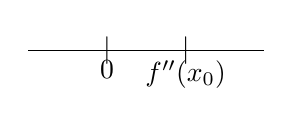
\begin{tikzpicture}
\draw (0,0)--(3,0);
\draw (1,0) node {$|$} node[below] {$0$};
\draw (2,0) node {$|$} node[below] {$f''(x_0)$};
\end{tikzpicture}\nl
Da $f'(x_0)=0$ ist, folgt:\\
$f'(x)>0$ auf $(x_0,x_0+\eps)$, das heißt, $f$ ist dort s.m.w.\\
$f'(x)<0$ auf $(x_0-\eps,x_0)$, das heißt, $f$ ist dort s.m.f.\\
$\Ra$ Behauptung. \qed\nl
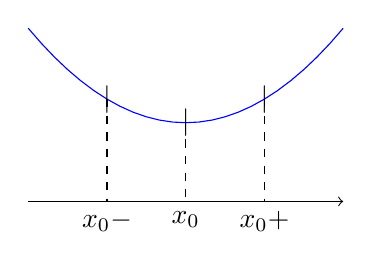
\begin{tikzpicture}
\draw[->] (-2,0)--(2,0);
\draw[color=blue,domain=-2:2] plot (\x, {0.3*abs(\x)^2+1});
\draw (0,1) node {$|$};
\draw (0,0) node[below] {$x_0$};
\draw[dashed] (0,1)--(0,0);
\draw (-1,1.3) node {$|$};
\draw (-1,0) node[below] {$x_0-\eps$};
\draw[dashed] (-1,1.3)--(-1,0);
\draw (1,1.3) node {$|$};
\draw (1,0) node[below] {$x_0+\eps$};
\draw[dashed] (1,1.3)--(1,0);
\end{tikzpicture}

\newpage

\section{Regel von de L'Hospital (nützliche Regel zur Berechnung von Grenzwerten)}\label{11.16}
$f, g: (a,b) \to \R$ seien differenzierbar, mit $g'(x) \neq 0 \forall x \in (a,b)$.\nl
Es gelte:
\enr{
\item $f(x) \to 0$ und $g(x) \to 0$ für $x \downarrow a$ \underline{oder}
\item $g(x) \to \pm \infty$ für $x \downarrow a$
}
$\Ra \lim_{x \downarrow a} \frac{f(x)}{g(x)} = \lim_{x \downarrow a} \frac{f'(x)}{g'(x)}$, sofern der Grenzwert rechts in $\R \cup \{\pm \infty\}$ existiert.\nl
Entsprechendes gilt für $x \uparrow b, x \to \pm \infty$

\subsection*{Beweis}
Hier ohne Beweis.

\subsection*{Beispiele}
\en{
\item $\lim_{x \to 0} \frac{\sin x}{x} \underset{\frac{0}{0}}{=} \lim_{x \to 0} \frac{\cos x}{1} = \cos 0 = 1$
\item $\lim_{x \to 0} \left(\frac{1}{x}-\frac{1}{\sin x}\right) = \lim_{x \to 0} \frac{\sin x - x}{x \cdot \sin x} \underset{\frac{0}{0}}{=} \lim_{x \to 0} \frac{\cos x - 1}{x \cdot \cos x + \sin x} \underset{\frac{0}{0}}{=} \lim_{x \to 0} \frac{- \sin x}{2 \cos x - x \cdot \sin x} \underset{\text{L'Hos.}}{=} 0$\\
Existenz des Grenzwerts ergibt sich "`von hinten nach vorne"'
\item $\lim_{x \to \infty} \frac{\ln x}{x^2} = \lim_{x \to \infty} \frac{\frac{1}{x}}{2x} = 0$
}

\section{Definition: Konvexität}\label{11.17}
Sei $D \subseteq \R$ Intervall.\\
$f: D \to \R$ ist \underline{konvex} $:\Lra \forall x,y \in D \wedge \lambda \in (0,1)$ gilt: $f'(\lambda x + (1-\lambda) y) \le \lambda \cdot f(x) + (1-\lambda)f(y)$\\
$f$ konkav auf $D$ $:\Lra$ "`$\ge$"' in obiger Ungleichung

\subsection*{Geometrische Darstellung von Konvexität}
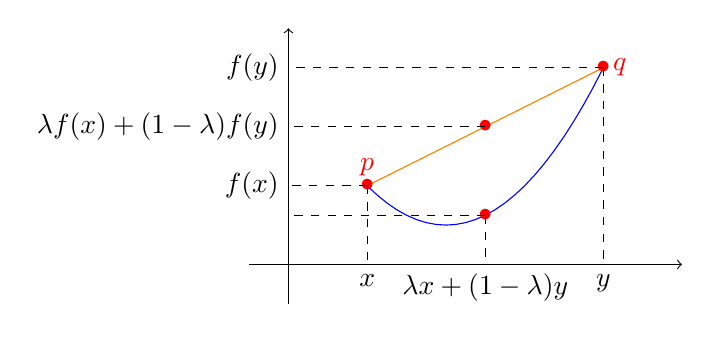
\begin{tikzpicture}
\draw[->] (-0.5,0)--(5,0);
\draw[->] (0,-0.5)--(0,3);
\draw[color=blue,domain=1:4] plot (\x, {0.5*abs(\x-2)^2+0.5}); % Graph f(x)
\draw[color=orange,domain=1:4] plot (\x, {0.5*\x+0.5}); % Sekante zwischen p und q
\draw[color=red] (1,1) node {$\bullet$} node[above] {$p$};
\draw[color=red] (4,2.5) node {$\bullet$} node[right] {$q$};
\draw[color=red] (2.5,0.625) node {$\bullet$};
\draw[color=red] (2.5,1.75) node {$\bullet$}; % Punkt auf Sekante
\draw[dashed] (1,1)--(1,0) node[below] {$x$};
\draw[dashed] (1,1)--(0,1) node[left] {$f(x)$};
\draw[dashed] (4,2.5)--(4,0) node[below] {$y$};
\draw[dashed] (4,2.5)--(0,2.5) node[left] {$f(y)$};
\draw[dashed] (2.5,0.625)--(2.5,0) node[below] {$\lambda x + (1-\lambda) y$};
\draw[dashed] (2.5,0.625)--(0,0.625);
\draw[dashed] (2.5,1.75)--(0,1.75) node[left] {$\lambda f(x) + (1-\lambda) f(y)$};
\end{tikzpicture}\nl
Die Sekante druch $p$ und $q$ liegt im Bereich $[x,y]$ oberhalb des Graphen von $f$

\newpage

\subsection*{Beispiele}
\en{
\item $f(x)=x^2$ ist konvex auf $\R$\nl
\begin{tikzpicture}
\draw[->] (-2,0)--(2,0);
\draw[->] (0,-0.5)--(0,2);
\draw[color=blue,domain=-1.41421:1.41421] plot (\x, {abs(\x)^2});
\end{tikzpicture}
\item \ \\
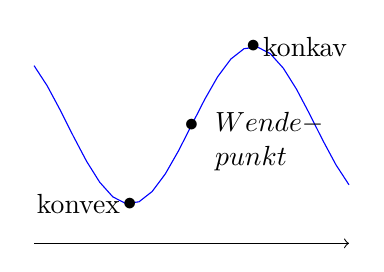
\begin{tikzpicture}
\draw[->] (-2,0)--(2,0);
\draw[color=blue,domain=-2:2] plot (\x, {sin(deg(2*\x))+1.5});
\draw (0,1.5) node {$\bullet$} node[right] {$\begin{array}{l} \ \\ \text{Wende-} \\ \text{punkt}\end{array}$}; % (vielleicht) mal schöner schreiben
\draw (0.78539,2.5) node {$\bullet$} node[right] {konkav};
\draw (-0.78539,0.5) node {$\bullet$} node[left] {konvex};
\end{tikzpicture}
}

\section{Konvexitätskriterium}\label{11.18}
Sei $f: (a,b) \to \R$ zwei mal differenzierbar, $-\infty \le a < b \le \infty$.\\
Dann gilt:
$$\begin{array}{l l l} f \text{ konvex} & \Lra & f'' \ge 0 \text{ auf } (a,b) \\ f \text{ konkav} & \Lra & f'' \le 0 \text{ auf } (a,b) \end{array}$$

\subsection*{Beweis}
Hier nur "`$\La$"' $f'' \ge 0 \Ra f'$ monoton wachsend auf $(a,b)$\\
Seien $x,y \in (a,b), \lambda \in (0,1), z := \lambda x + (1-\lambda)y$\\
$\frac{f(z)-f(x)}{z-x} \underset{\text{MWS}}{=} f'(\xi)$ mit $\xi \in (x,z)$, $\frac{f(y)-f(z)}{y-z} \underset{\text{MWS}}{=} f'(\eta), \eta \in (z,y)$, insbes.: $\xi < \eta$\\
$f'$ monoton $\Ra f'(\xi) \le f(\eta)$\\
$z-x = (1-\lambda)(y-x)$; $y-z = \lambda(y-x)$\\
$\Ra \frac{f(z)-f(x)}{1-\lambda} < \frac{f(y)-f(z)}{\lambda}$\\
$\Ra f(z) \left(\frac{1}{1-\lambda} + \frac{1}{\lambda}\right) \le \frac{f(x)}{1-\lambda} + \frac{f(y)}{\lambda}$\\
$\Ra f(z) = \lambda f(x) + (1-\lambda) f(y)$ \qed

\chapter{Trigonometrische Funktionen; Polarkoordinaten}\label{P12}
Erinnerung (Kapitel \ref{P8}): $x \in \R \Ra |e^{ix}| = 1$\nl
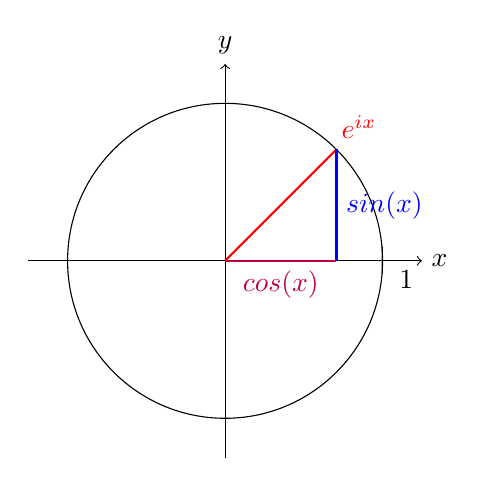
\begin{tikzpicture}
\draw[->] (-2.5,0)--(2.5,0) node[right] {$x$};
\draw[->] (0,-2.5)--(0,2.5) node[above] {$y$};
\draw (0,0) circle(2);
\draw[thick,color=red] (0,0)--(1.4142,1.4142);
\draw[color=red] (1.7,1.7) node {$e^{ix}$};
\draw[thick,color=blue] (1.4142,0)--(1.4142,1.4142);
\draw[color=blue] (1.4142,0.7071) node[right] {$sin(x)$};
\draw[thick,color=purple] (0,0)--(1.4142,0);
\draw[color=purple] (0.7071,0) node[below] {$cos(x)$};
\draw (2,0) node{$|$};
\draw (2.3,0) node[below]{$1$};
\end{tikzpicture}\nl
$\cos x = \RE(e^{ix}) = \frac{e^{ix}+e^{-ix}}{2}$\\
$\sin x = \IM(e^{ix}) = \frac{e^{ix}-e^{-iy}}{2i}$\\
$\cos^2 x + \sin^2 x = |e^{ix}|^2 = 1$\nl
$\sin, \cos$ sind differenzierbar auf $\R$, $\sin'=\cos, \cos'=-\sin$

\section{Satz + Definition}\label{12.1}
$\cos x$ hat auf $[0,2]$ genau eine Nullstelle. Diese wird mit $\frac{\pi}{2}$ bezeichnet.\nl
$\pi$ ist die \underline{Kreiszahl}, $\pi \approx 3,14159\ldots$\\
$\pi$ ist irrational, sogar \href{https://de.wikipedia.org/wiki/Transzendente_Zahl}{\underline{transzendent}}.

\newpage

\subsection*{Beweis}
$\cos 0 = 1 > 0$\\
Einschließungslemma: $x \in [0,2] \Ra \cos x \le 1 - \frac{x^2}{2} + \frac{x^4}{24}$\\
$\Ra \cos 2 \le 1 - \frac{4}{2} + \frac{16}{24} < 0$\\
ZWS $\Ra \cos$ hat mindestens eine Nullstelle in $[0,2]$\nl
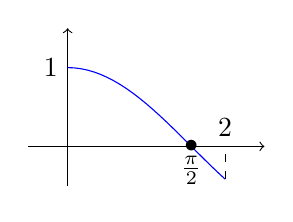
\begin{tikzpicture}
\draw[->] (-0.5,0)--(2.5,0);
\draw[->] (0,-0.5)--(0,1.5);
\draw[color=blue,domain=0:2] plot (\x, {cos(deg(\x))});
\draw (1.57079,0) node {$\bullet$} node[below] {$\frac{\pi}{2}$};
\draw (0,1) node[left] {$1$};
\draw (2,0) node[above] {$2$};
\draw[dashed] (2,-0.41614)--(2,0);
\end{tikzpicture}\nl
$x \in (0,2] \underset{\text{Einschl.}}{\Ra} \sin x \ge x \cdot \left(1-\frac{x^2}{6}\right) > 0 \Ra \cos'x = - \sin x < 0$ auf $(0,2]$\\
$\underset{\text{\ref{11.13}}}{\Ra} \cos x$ ist streng monoton fallend auf $(0,2] \Ra$ hat nur eine Nullstelle \qed\nl
$\cos \frac{\pi}{2} = 0 \Ra \sin \frac{\pi}{2} = 1$ (da $\sin > 0$ auf $(0,2]$)\\
$\Ra e^{i \cdot \frac{\pi}{2}} = \cos \frac{\pi}{2} + i \cdot \sin \frac{\pi}{2} = i$\\
FG für $\exp \Ra e^{i \pi} = \left(e^{i \frac{\pi}{2}}\right)^2 = -1$, etc.\nl
\underline{Wertetabelle}:\\
\begin{tabular}{c||c|c|c|c}
$x$ & $\frac{\pi}{2}$ & $\pi$ & $\frac{2 \pi}{2}$ & $2 \pi$ \\ 
\hline $e^{ix}$ & $i$ & $-1$ & $-i$ & $1$ \\ 
\hline $\cos x$ & $0$ & $-1$ & $0$ & $1$ \\ 
\hline $\sin x$ & $1$ & $0$ & $-1$ & $0$
\end{tabular}\nl
\begin{tikzpicture}
\draw[->] (-2.5,0)--(2.5,0);
\draw[->] (0,-2.5)--(0,2.5);
\draw[color=blue] (0,0) circle(2);
\draw (1.7,0) node[below]{$1$};
\draw[color=red] (2,0) node {$\bullet$};
\draw[color=red] (2,0.3) node[right] {$e^{2 i \pi} = e^0$};
\draw[color=red] (-2,0) node {$\bullet$};
\draw[color=red] (-2,0.3) node[left] {$e^{i \pi}$};
\draw[color=red] (0,2) node {$\bullet$};
\draw[color=red] (0,2.3) node[right] {$e^{\frac{i \pi}{2}}$};
\draw[color=red] (0,-2) node {$\bullet$};
\draw[color=red] (0,-2.3) node[right] {$e^{\frac{3 i \pi}{2}} = e^{-\frac{i \pi}{2}}$};
\end{tikzpicture}\nl
$e^{2 i \pi} = 1 \underset{\text{FG}}{\Ra} e^{z+2 i \pi} \underset{\text{FG}}{=} e^z \forall z \in \C$

\section{Korollar: Periodizität von exp}\label{12.2}
$z \in \C \Ra$ \fbox{$e^{z + 2 \pi i} = e^z$}\\
$e^{z + i \pi} = -e^z$\\
$e^{z \pm \frac{i \pi}{2}} = \pm i e^z$\nl
$z = ix, x \in \R \Ra e^{i(x+2\pi)} = e^{ix}$; $e^{i(x+\pi)} = -e^{ix}$; $e^{i(x+\frac{\pi}{2})} = \pm ie^{ix}$\nl
Zerlege in Real- und Imaginärteile:

\section{Korollar}\label{12.3}
$\cos(x+2\pi) = \cos x$\\
$\sin(x+2\pi) = \sin x$\\
$\cos, \sin$ sind \underline{$2\pi$-periodisch}\nl
Ferner:\\
$\cos(x+\pi) = -\cos x$; $\sin(x+\pi) = -\sin x$; $\cos(x \pm \frac{\pi}{2}) = \mp \sin x$; $\sin(x \pm \frac{\pi}{2}) = \pm \cos x$

\section{Satz}\label{12.4}
$\cos$ hat auf $\R$ genau die Nullstellen $\frac{\pi}{2}+k \pi, k \in \Z$\\
$\sin$ hat auf $\R$ genau die Nullstellen $k \pi, k \in \Z$\nl
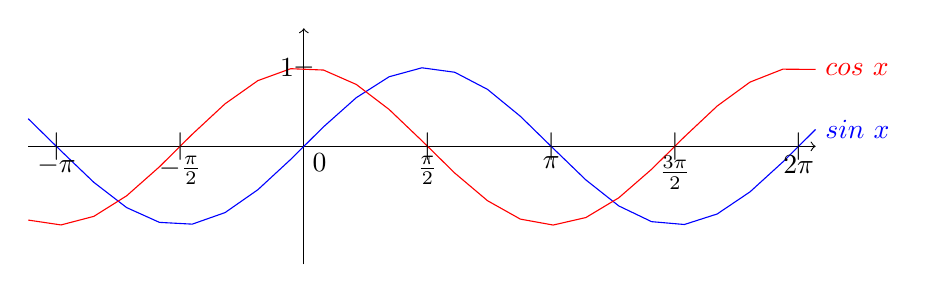
\begin{tikzpicture}
\draw[->] (-3.5,0)--(6.5,0);
\draw[->] (0,-1.5)--(0,1.5);
\draw[blue, domain=-3.5:6.5] plot (\x, {sin(deg(\x))}) node[right] {$sin \ x$};
\draw[red, domain=-3.5:6.5] plot (\x, {cos(deg(\x))}) node[right] {$cos \ x$};
\draw (0,1) node{$-$} [left] node{$1$};
\draw (0.2,-0.2) node{$0$};
\draw (-3.1415927,0) node{$|$} [below] node{$-\pi$};
\draw (-1.5707963,0) node{$|$} [below] node{$-\frac{\pi}{2}$};
\draw (1.5707963,0) node{$|$} [below] node{$\frac{\pi}{2}$};
\draw (3.1415927,0) node{$|$} [below] node{$\pi$};
\draw (4.712389,0) node{$|$} [below] node{$\frac{3\pi}{2}$};
\draw (6.2831853,0) node{$|$} [below] node{$2\pi$};
\end{tikzpicture}

\subsection*{Beweis}
$\cos(-x)=\cos x \Ra \cos$ hat auf $(-\frac{\pi}{2}, \frac{\pi}{2})$ nur $\frac{\pi}{2}$ als Nullstelle. $\cos(x+\pi) = -\cos x$\\
$\Ra$ auf $(-\frac{\pi}{2}, \frac{3 \pi}{2}]$ hat es genau die Nullstellen $\frac{\pi}{2}, \frac{3 \pi}{2}$\\
$2 \pi$-Periodizität $\Ra$ Behauptung für $\cos$.\\
Für $\sin$ folgt daraus wegen $\sin(x+\frac{\pi}{2}) = \cos x$ \qed